%%
%% This is file `sample-sigconf.tex',
%% generated with the docstrip utility.
%%
%% The original source files were:
%%
%% samples.dtx  (with options: `sigconf')
%%
%% IMPORTANT NOTICE:
%%
%% For the copyright see the source file.
%%
%% Any modified versions of this file must be renamed
%% with new filenames distinct from sample-sigconf.tex.
%%
%% For distribution of the original source see the terms
%% for copying and modification in the file samples.dtx.
%%
%% This generated file may be distributed as long as the
%% original source files, as listed above, are part of the
%% same distribution. (The sources need not necessarily be
%% in the same archive or directory.)
%%
%% The first command in your LaTeX source must be the \documentclass command.
\documentclass[sigconf,10pt]{acmart}

\settopmatter{printfolios=true}

\usepackage{hyperref}


\providecommand{\tightlist}{%
  \setlength{\itemsep}{0pt}\setlength{\parskip}{0pt}}

%%
%% \BibTeX command to typeset BibTeX logo in the docs
\AtBeginDocument{%
  \providecommand\BibTeX{{%
    \normalfont B\kern-0.5em{\scshape i\kern-0.25em b}\kern-0.8em\TeX}}}

%% Rights management information.  This information is sent to you
%% when you complete the rights form.  These commands have SAMPLE
%% values in them; it is your responsibility as an author to replace
%% the commands and values with those provided to you when you
%% complete the rights form.


%%
%% Submission ID.
%% Use this when submitting an article to a sponsored event. You'll
%% receive a unique submission ID from the organizers
%% of the event, and this ID should be used as the parameter to this command.
%%\acmSubmissionID{123-A56-BU3}

%%
%% The majority of ACM publications use numbered citations and
%% references.  The command \citestyle{authoryear} switches to the
%% "author year" style.
%%
%% If you are preparing content for an event
%% sponsored by ACM SIGGRAPH, you must use the "author year" style of
%% citations and references.
%% Uncommenting
%% the next command will enable that style.
%%\citestyle{acmauthoryear}

%%
%% end of the preamble, start of the body of the document source.
\begin{document}

%%
%% The "title" command has an optional parameter,
%% allowing the author to define a "short title" to be used in page headers.
\title{A Unified Interaction Model For Web Scraping \& Customization}

%%
%% The "author" command and its associated commands are used to define
%% the authors and their affiliations.
%% Of note is the shared affiliation of the first two authors, and the
%% "authornote" and "authornotemark" commands
%% used to denote shared contribution to the research.

\author{Kapaya Katongo}
\affiliation{%
  \institution{MIT CSAIL}
  \city{Cambridge, MA}
  \country{USA}
}
\email{kkatongo@mit.edu}

\author{Geoffrey Litt}
\affiliation{%
  \institution{MIT CSAIL}
  \city{Cambridge, MA}
  \country{USA}
}
\email{glitt@mit.edu}

\author{Kathryn Jin}
\affiliation{%
  \institution{MIT CSAIL}
  \city{Cambridge, MA}
  \country{USA}
}
\email{kjin@mit.edu}

\author{Daniel Jackson}
\affiliation{%
  \institution{MIT CSAIL}
  \city{Cambridge, MA}
  \country{USA}
}
\email{dnj@csail.mit.edu}

%%
%% By default, the full list of authors will be used in the page
%% headers. Often, this list is too long, and will overlap
%% other information printed in the page headers. This command allows
%% the author to define a more concise list
%% of authors' names for this purpose.
% \renewcommand{\shortauthors}{Trovato and Tobin, et al.}

%%
%% The abstract is a short summary of the work to be presented in the
%% article.
\begin{abstract}
  Web scraping, the process of extracting structured data from a
  website, is a common building block of web customization systems.
  Prior approaches have allowed users to perform web scraping by
  directly demonstrating examples of the data to scrape. However,
  demonstrations alone do not allow for as much expressiveness as
  traditional programming which is vital for complex web scraping tasks.

  In this paper, we present a new interaction model for web scraping
  that combines the ease of use of programming-by-demonstration and the
  expressiveness of traditional programming. When a user demonstrates
  examples of data to extract, a web scraping program is synthesized and
  presented as a spreadsheet formula. Crucially, the user can directly
  edit and execute the formula using pure functional semantics, allowing
  them to specify scraping operations which can not be achieved via
  demonstration alone.

  To illustrate our model, we implement it as a browser extension called
  Joker. Through concrete examples, a small user study and a cognitive
  dimenions of notation analysis, we show how Joker offers more
  expressive web scraping and customization than prior systems.
\end{abstract}

%%
%% The code below is generated by the tool at http://dl.acm.org/ccs.cfm.
%% Please copy and paste the code instead of the example below.
%%
%% From HERE
\begin{CCSXML}
<ccs2012>
<concept>
<concept_id>10011007.10011006.10011066.10011069</concept_id>
<concept_desc>Software and its engineering~Integrated and visual development environments</concept_desc>
<concept_significance>500</concept_significance>
</concept>
</ccs2012>
\end{CCSXML}

\ccsdesc[500]{Software and its engineering~Integrated and visual development environments}
% To HERE

%%
%% Keywords. The author(s) should pick words that accurately describe
%% the work being presented. Separate the keywords with commas.
\keywords{end-user programming, software customization, web scraping, programming-by-example, program synthesis}

%% A "teaser" image appears between the author and affiliation
%% information and the body of the document, and typically spans the
%% page.
%\begin{teaserfigure}
%  \includegraphics[width=\textwidth]{sampleteaser}
%  \caption{Seattle Mariners at Spring Training, 2010.}
%  \Description{Enjoying the baseball game from the third-base
%  seats. Ichiro Suzuki preparing to bat.}
%  \label{fig:teaser}
%\end{teaserfigure}

%%
%% This command processes the author and affiliation and title
%% information and builds the first part of the formatted document.
\maketitle

\hypertarget{sec:introduction}{%
\section{Introduction}\label{sec:introduction}}

Many websites on the internet do not meet the exact needs of all of
their users. Because of this, millions of people use browser extensions
like Greasemonkey \citep{zotero-224} and Tampermoneky \citep{zotero-191}
to install userscripts, snippets of Javascript code which customize the
behavior of websites. To make the creation of web customizations more
accessible to end-users without knowledge of programming, researchers
have developed systems like Sifter \citep{huynh2006}, Vegemite
\citep{lin2009} and Wildcard \citep{litt2020, litt2020b}.

A common building block of these web customization systems is web
scraping, the extraction of structured data from websites. They achieve
web scraping in one of two ways: programming-by-demonstration
\citep{huynh2006, lin2009} and traditional programming
\citep{litt2020, litt2020b}. Web scraping by demonstration automates the
web scraping process by utilizing program synthesis to synthesize a web
scraping program from user demonstrations. This approach is accessible
to end-users with no programming experience and enables them to fully
participate in the customization lifecycle. However, web scraping by
demonstration is not powerful enough to perform complex web scraping
tasks. On the other side, web scraping by programming involves
programmers manually writing web scraping code. It allows for scraping a
wider variety of websites but is not accessible to end-users who can
only customize websites that programmers have written web scraping code
for.

In this paper, we present a new interaction model for web scraping for
customization that combines the ease of use of
programming-by-demonstration and the expressiveness of traditional
programming. At its core lies a simple formula language. The language
offers pure functional semantics for expressing and executing data
extractions from websites using Cascading Style Sheet (CSS) selectors.
When a user demonstrates examples of data to scrape, a web scraping
program is synthesized via wrapper induction \citep{kushmerick2000} and
is presented as a formula containing the CSS selector required to scrape
the data (Section~\ref{sec:implementation}). Cruicially, the formula can
be directly edited and executed to specify complex scraping operations
which can not be achieved by demonstrations alone. This interaction
model coupled with live, intermediate results of operations offers a
tight feedback loop that supports exploratory and incremental web
scrapping.

We have implemented this new model of web scraping as an extension of
Wildcard \citep{litt2020, litt2020b} called Joker. Wildcard enables web
customization by direct manipulation of a spreadsheet-like table it adds
to websites. The table contains the website's underlying structured data
and is bidirectionally synchronized with it. User interactions with the
table, including sorting, adding columns and running computations in a
spreadsheet formula language, are propagated to the website thereby
customizing it. The web scraping required to create Wildcard's table can
only be achieved via traditional programming in Javascript. This means
that end-users can only customize websites that programmers have written
web scraping code for. Joker enables end-users to achieve the web
scraping tasks required for customization while maintaining some of the
expressivness of traditional programming.

By representing demonstrations as formulas, our new web scraping
interaction model fit right into Wildcard's customization paradigm which
utilizes formulas for web customization. This enabled us to go beyond
providing an interaction model that combines web scraping by
demonstration with web scraping by programming to providing an
interaction model that combines web scraping \emph{and} customization.
We refer to this as a \emph{unified interaction model for web scraping
and customization}. In Section~\ref{sec:examples}, we show how this
offers more expressive web scraping and customization than prior
systems.

Our contributions are as follows:

\begin{itemize}
\tightlist
\item
  A \textbf{unified interaction model for web scraping and
  customization} that combines web scraping (by demonstration and
  programing) with web customization through a shared formula language
  with pure functional semantics
\item
  An implementation of the unified interaction model for web scraping
  and customization called Joker that combines three key design
  principles (\textbf{mixed-initiative interaction}, \textbf{functional
  reactive programming} \& \textbf{unified user interaction}) in a novel
  way (Section~\ref{sec:design-principles})
\item
  The results of an evaluation of the model via an example gallery, a
  five person user study and a cognitive dimensions of notion analysis
  (Section~\ref{sec:evaluation})
\end{itemize}

We end by discussing opportunities for future work
(Section~\ref{sec:conclusion}).

\hypertarget{sec:examples}{%
\section{Example Usage Scenario}\label{sec:examples}}

To concretely illustrate the user experience of our tool, we present a
scenario of customizing eBay, a popular online marketplace. The goal of
the user, Jen, is to filter out search results that are sponsored,
i.e.~product listings that a seller paid to promote. On the webpage,
sponsored listings are marked with a ``Sponsored'' label that Jen can
try to scrape, then she can sort the scraped labels to move all
sponsored listings to the bottom of the page. Figure~\ref{fig:ebay}
shows accompanying screenshots.

\begin{figure*}
  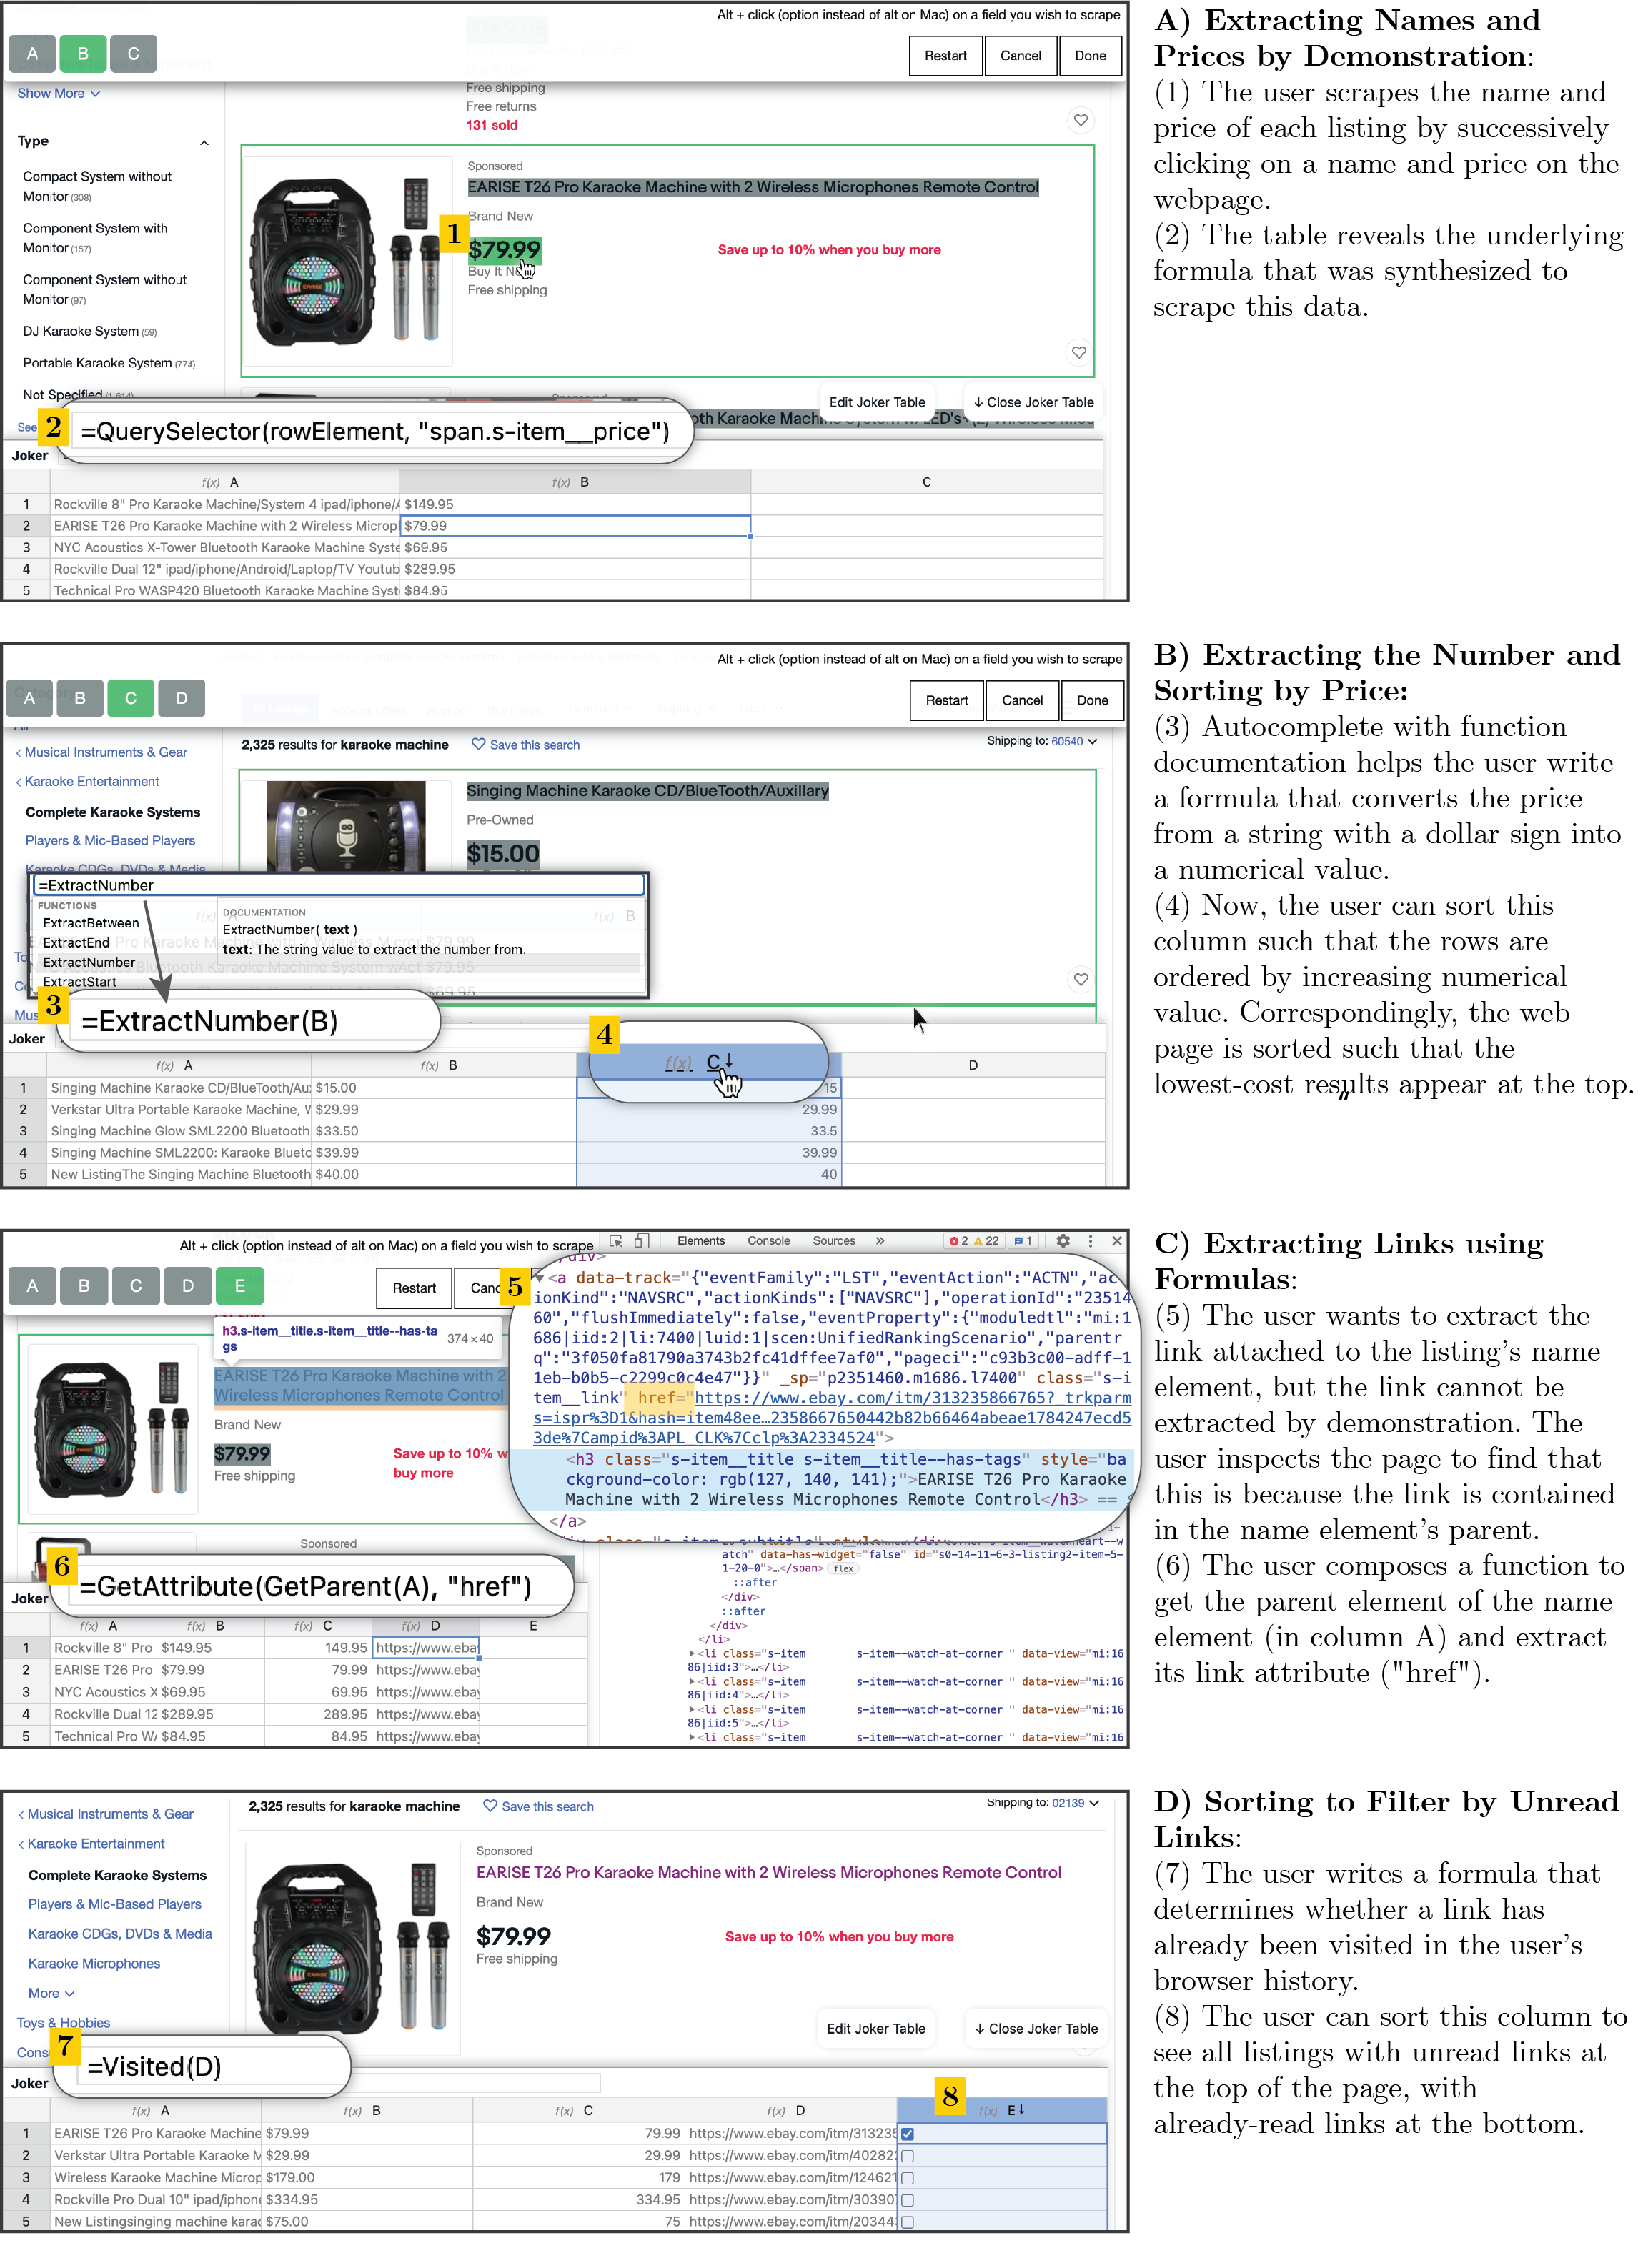
\includegraphics[width=\textwidth]{media/ebay.png}
  \caption{\label{fig:ebay}Scraping and customizing eBay by unified demonstration and formulas.}
\end{figure*}

\textbf{Scraping Names by Demonstration} (Figure~\ref{fig:ebay} Part A):
Jen starts the adapter creation process by clicking a context menu item
within the eBay.com page, then hovering over the data that she would
like to scrape: the page element that contains the name of the listing.
The system provides live feedback as Jen hovers: it annotates the row of
data with a border, highlights the column of data in the page with a
green background, and displays how the values will appear in the data
table. When she clicks, the highlighted data is saved into the table.

The text content of the highlighted element is now displayed in the
first column of the table, with one cell for each listing containing the
name of the listing. When she clicks on a cell, Jen can see that the
textual data is also represented by a formula:

\texttt{QuerySelector(rowElement,\ "h3.s-item\_\_title")}

This formula reveals how Joker is actually scraping this column's data
behind the scenes: it calls a query selector on each listing (i.e.~each
\texttt{rowElement}) on the page. Scraped data is stored as functions
that act on the data on the page, instead of as static text, based on
our design principle of \textbf{functional reactive programming}. Joker
exposes this formula to the user to exemplify how scraping is achieved
with formulas and to provide a template for scraping with formulas.

After this first demonstration, Jen has a reference to each of the
page's row elements (i.e.~each product listing) in the Joker table. She
can now use these references to scrape elements within the product
listing with formulas, such as the Sponsored label.

\textbf{Scraping Sponsored Labels with Formulas} (Figure~\ref{fig:ebay}
Part B): Next, Jen attempts to scrape contents of the ``Sponsored''
label element into a new column; having this column would allow her to
sort the table based on whether the listing contains the ``Sponsored''
label. She tries to scrape the label using demonstration, but she is
unable to scrape more than one letter of the word at a time. To diagnose
the issue, Jen inspects the page's source code using her browser's
developer tools. Jen discovers that eBay's developers have inserted
invisible letters into word ``Sponsored'' (possibly to obfuscate against
ad blockers). Each letter is in its own HTML element, and the inserted
letters are rendered invisible by CSS. Scraping by demonstration does
not work in this case because Jen wants the element that contains the
whole word, but the system is giving her the leaf-node elements
(individual letters) instead.

Jen sees in the source code that the all of the letters of the
``Sponsored'' label, both visible and invisible, are contained in a
single ancestor element with the CSS selector
\texttt{"div.s-item\_\_title-\/-tagblock"}. Thus, she is able to scrape
the full word by writing a query selector formula with with that CSS
selector. She can copy the formula from the previous column as a
template. The resulting formula is

\texttt{QuerySelector(rowElement,\ "div.s-item\_\_title-\/-tagblock")}

This formula populates the column with the text content of the
``Sponsored'' element, which she can now use for string manipulation and
sorting. By writing a formula, Jen is able to overcome the limitations
of scraping by demonstration. The mixed methods of scraping exemplify
our tool's support of \textbf{mixed-initiative interaction}.

\textbf{Filtering Sponsored Results} (Figure~\ref{fig:ebay} Part C): The
query selector that Jen just wrote returns all of the text within each
of the targeted ``Sponsored'' elements, including any invisible letters.
eBay's web design is that sponsored listings have a visible
``Sponsored'' label with invisible inserted letters, and non-sponsored
listings have an invisible ``Sponsored'' label. Thus, for sponsored
listings, the query returns garbled text
(e.g.~``JSp3onMsoV3rXNYFedZB''), and for non-sponsored listings, the
query returns ``Sponsored.'' Jen identifies this correlation by
scrolling through the scraped data in the column and comparing them to
what she sees on the web page. Then, in a new column, Jen writes a
formula that returns whether or not the previous column's text includes
the word ``Sponsored.'' Finally, she sorts the listings by whether or
not they are sponsored by sorting this column, thus hiding sponsored
results from view. This customization is possible because Joker provides
a \textbf{unified user model}, where scraping and customization are
performed in conjunction.

In this way, Jen is able to use our system to customize the eBay
website, without needing to learn how to program in JavaScript and
without even leaving the webpage. Our model of customization by unified
demonstration and formulas is flexible enough to support a wide range of
other useful modifications and web programming proficiency levels, and
we present a greater variety of use cases in
Section~\ref{sec:evaluation}.

\hypertarget{sec:implementation}{%
\section{System Implementation}\label{sec:implementation}}

In this section, we outline the \emph{wrapper induction}
\citep{kushmerick2000} algorithm that Joker uses to synthesize web
scraping programs from user demonstrations. Then, we briefly describe
the formula language used to represent the sythesized web scraping
programs and include a list of the formulas that are currently available
and their roles.

\hypertarget{wrapper-induction}{%
\subsection{Wrapper Induction}\label{wrapper-induction}}

In order to create web scraping programs from users demonstrations,
Joker solves the wrapper induction \citep{kushmerick2000} task:
generalizing from a few examples of data in a data set to a
specification that specifies the all the data in the data set.

Joker takes an approach similar to that used in systems like Vegemite
\citep{lin2009} and Sifter \citep{huynh2006}. It synthesizes a single
\emph{row selector} for the website: a CSS selector that identifies a
set of DOM elements corresponding to the rows of the data set. For each
column in the data set, it synthesizes a \emph{column selector}, a CSS
selector that identifies the element containing the column value.

One important difference is that our algorithm only accepts row elements
that have direct siblings with a similar structure. We refer to this as
the \emph{row-sibling} constraint. Later, we describe how this
constraint provides a useful simplification of the wrapper induction
task and in \citep{section:evaluation} discuss the resulting limitations
this puts on our system. We proceed to describe how CSS selectors are
synthesized for row and column elements and then explain the criteria
used to determine row elements.

\hypertarget{synthesizing-css-selectors}{%
\subsubsection{Synthesizing CSS
Selectors}\label{synthesizing-css-selectors}}

Joker synthesizes two types of CSS selectors: a single row selector that
selects a set of DOM elements corresponding to the rows of the data set
and a column selector for each column which selects the element
containing the column value within a given row.

For a given row element, its row selector is synthesized using the
following criteria:

\emph{Plausibility}. A selector is a plausible row selector if it 1)
consists of a subset of the classes on the row element and 2) consists
of a subset of the classes all the row element's siblings. The second
point is the \emph{row-sibling} constraint we mentioned. Notice how it
simplifies the problem by eliminating selectors.

\emph{Weight}. A selector has a weight equal to the number of classes it
consists of.

\emph{Best}. A selector is the best if it is plausible and there is no
other selector that has a lower weight than it has. We favor selectors
with the lowest weight to ensure that only the mininum required classes
are utlized. If there are multiple selectors that are plausible and have
the lowest weight, we only pick one.

For a given column element, its column selector is synthesized using the
following criteria:

\emph{Plausibility}. A selector is a plausible column selector if it 1)
consists of a subset of the classes on the column element and 2) only
selects the give column element when applied on the corresponding row
element.

\emph{Weight}. A selector has a weight equal to the number of classes it
consists of.

\emph{Best}. A selector is the best if it is plausible and there is no
other selector that has a lower weight than it has. As before, we favor
selectors with the lowest weight and only pick one if there are multiple
that fulfil the criteria.

One aspect of future work is saving the list of all selectors that fufil
the criteria and making them available to users to view and pick from.
This would be similar to Mayer et el's user interaction model called
\emph{program navigation} \citep{mayer2015} that gives users the
opportunity to navigate all valid, synthesized programs and pick the
best one.

\hypertarget{determing-row-elements}{%
\subsubsection{Determing Row Elements}\label{determing-row-elements}}

When a user first demonstrates a column value, Joker uses the
demonstration to synthesize a row selector that will identify all the
row elements in the website and a column selector that will identify the
element that contains the column value. During subsequent
demonstrations, Joker simply synthesizes a column selector for the
column element that contains the demonstrated column value. Like similar
approaches \citep{huynh2006, lin2009, chasins2018}, all demonstrations
have to be made from the same row element.

Given a demonstrated column value, row elements are determined using the
following criteria:

\emph{Plausibility}. An element \texttt{R} is a plausible row element if
1) it is within the \texttt{body} element of the DOM, 2) it is in the
parent path of the column element \texttt{C} containing the demonstrated
column value \texttt{V} and 3) the CSS selector \texttt{S} of element
\texttt{C} only identifies \texttt{C} when applied it.

\emph{Weight}. A row element \texttt{R} is has a weight \texttt{W} equal
to the number of its siblings for which the CSS selector \texttt{S} of
column element \texttt{C} only identifies \texttt{C} when applied to
it`.

\emph{Best}. A row element \texttt{R} is the best if it is plausible and
there is no other row element that has a higher weight than it. We favor
row elements with the highest weight ensure that we end up with a data
set with the highest number of column values corresponding to
\texttt{V}. If there are multiple plausible row elements with the
highest weight, we pick the one closet to the column element \texttt{C}
in its parent path.

Figure~\ref{fig:algorithm} provides a concrete example of how the above
criteria are applied to determine a row element from the demonstration
of a column value.

\begin{figure*}
  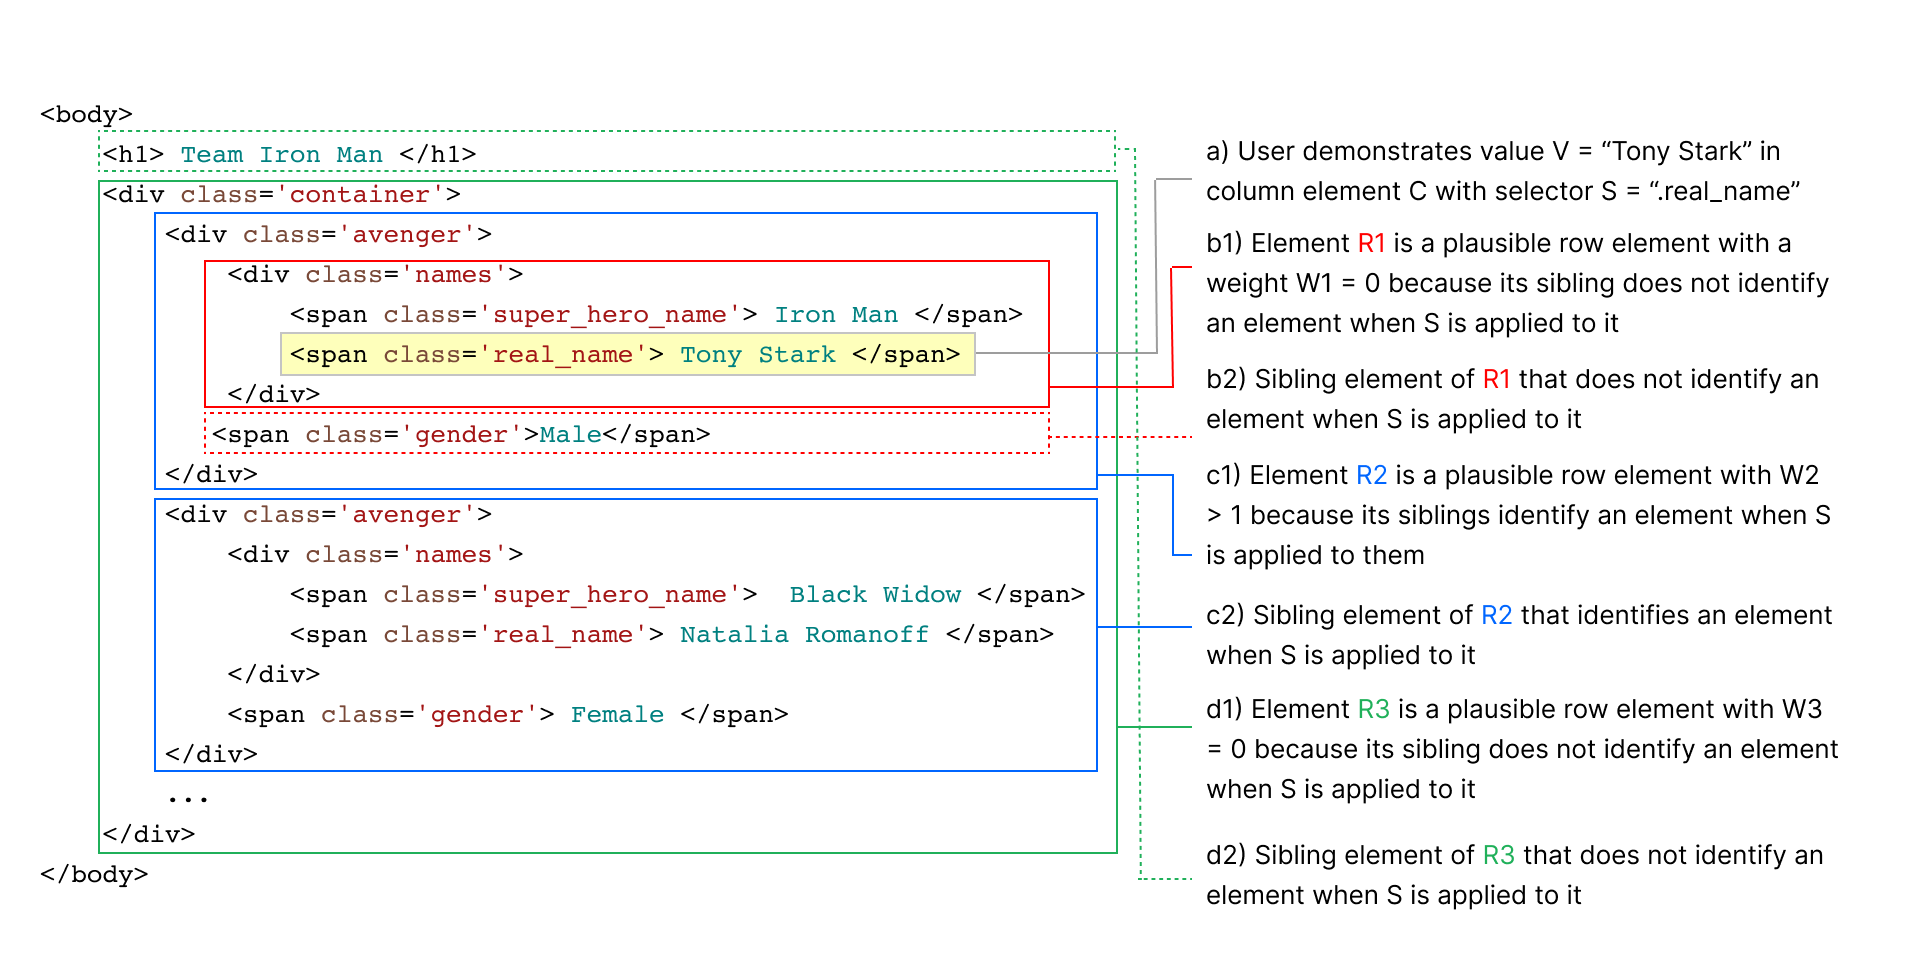
\includegraphics[width=\textwidth]{media/algorithm.png}
  \caption{\label{fig:algorithm} A example of how Joker's wrapper indunction algorithm is used to determine the row element from the demonstration of a column value. The row element is correctly determind to be R2.}
\end{figure*}

\hypertarget{web-scraping-formulas}{%
\subsection{Web Scraping Formulas}\label{web-scraping-formulas}}

Joker's formula language is similar to that of visual database query
systems like SIEUFERD \citep{bakke2016} and Airtable \citep{zotero-228}.
Formulas automatically apply across an entire column of data and
reference other column names instead of values in specific rows. This is
more efficient than users having to copy a formula across a column as in
traditional spreadsheets like Microsoft Excel and Google Sheets. It of
course comes at the cost of not being able to specify a formula for only
a subset of column cells but this hasn't yet come up in our use cases.
The language currently consists of the following formulas:

\hypertarget{queryselectorrowelement-selector}{%
\subsubsection{QuerySelector(rowElement,
selector)}\label{queryselectorrowelement-selector}}

This formula is used to represent the web scraping program synthesized
from demonstrations. \texttt{rowElement} is a special keyword that
reference a hidden column containing the DOM elements that correspond to
the rows of the data set. \texttt{selector} is the synthesized CSS
selector that specifices which elemnt to scrape data from.

\hypertarget{getparentelement}{%
\subsubsection{GetParent(element)}\label{getparentelement}}

This formula is used to traverse the DOM when the data to be scraped is
made of the values of its containing and sibling elements.
Demonstrations alone cannot be used to scrape such data.
\texttt{element} can be a reference to a column containing a
\texttt{QuerySelector} formula (\texttt{GetParent(A)}) or a
\texttt{QuerySelector} formula itself
(\texttt{=GetParent(QuerySelector(...))}).

\hypertarget{getattributeelement-attribute}{%
\subsubsection{GetAttribute(element,
attribute)}\label{getattributeelement-attribute}}

This formula is used to scrape data from DOM attributes. An example of
this are URLs which are available on the \texttt{href} attribute of link
elements. \texttt{element} is as described for \texttt{GetParent} and
\texttt{attribute} is the name of the attribute to scrape
(\texttt{GetAttribute(A,\ "href")}).

\hypertarget{sec:design-principles}{%
\section{Design Principles}\label{sec:design-principles}}

Below, we describe three design principles that the implementation of
our model embodies. We did not invent these principles but rather
combined them in a novel manner for the domain of web scraping and web
customization.

\hypertarget{mixed-initiative-interaction}{%
\subsection{Mixed-Initiative
Interaction}\label{mixed-initiative-interaction}}

In a position paper \citep{chugh2016a}, Chugh discusses how programmatic
and direct manipulation systems each have distinct strengths but users
are often forced to choose one over another. As a solution, he makes a
proposal for ``novel software systems that tightly couple programmatic
and direct manipulation'' which led to the emergence of systems like
Sketch-N-Sketch \citep{chugh2016}. More generally, this idea relates to
work on mixed-initiative interaction by Horvitz \citep{horvitz1999} in
which he advocates for ``designs that take advantage of the power of
direct manipulation and potentially valuable automated reasoning.'' In
our system, mixed-initiative interaction refers to the fluid
interleaving of programming-by-demonstration and traditional programming
for web scraping.

This type of mixed-initiative interaction can be seen in a number of
programming-by-example systems. Sketch-N-Sketch \citep{chugh2016} allows
users to create an SVG shape via traditional programming and then switch
to modifying its size or shape via direct manipulation. Wrex
\citep{drosos2020} takes examples of data transforms and generates
readable and editable Python code. Small-Step Live Programming By
Example \citep{ferdowsifard2020} presents a paradigm in which
programming-by-example is used to synthesize small parts of a user
authored program instead of delegating construction of entire program.
Mayer et al \citep{mayer2015} developed a user interaction model called
\emph{program navigation} which allows users to navigate between all
synthesized programs instead of only displaying the top-ranked one.

Our unified model for web scraping and customization offers
mixed-initiative interaction by presenting the result of
programming-by-demonstration as a formula. This is advantageous as it
not only allows users to delegate automation to the system via
demonstrations but also allows users to modify the output of the
demonstration. In the Ebay example in Section~\ref{sec:examples}, the
user starts out by demonstrating to scrape, switches to manually
authoring a web scraping formula when demonstrating is insufficient and
then switches back to demonstrating, all in a seamless and fluid manner.

\hypertarget{functional-reactive-programming}{%
\subsection{Functional Reactive
Programming}\label{functional-reactive-programming}}

In general terms, functional reactive programming (FRP) is the
combination of functional and reactive programming: it is functional in
that it uses functions to define programs that manipulate data and
reactive in that it defines data flows through which changes in data are
propagated. FRP has seen wide adoption in end-user programming through
implementations such as spreadsheet formula languages (Microsoft Excel
\& Google Sheets) and formula languages for low-code programming
environments (Microsoft Power Fx \citep{zotero-150}, Google AppSheet
\citep{zotero-218}, Airtable \citep{zotero-228}, Glide
\citep{zotero-148}, Coda \citep{zotero-155} \& Gneiss
\citep{chang2014}).

Wildcard \citep{litt2020, litt2020b} already provided functional
reactive programming via a spreadsheet formula language aimed at
increasing the expressiveness of customizations. The language has
formulas to encapsulate logic, perform operations on strings, call
browser APIs and even invoke web APIs. As per the FRP paradigm, users
only have to think in terms of operations on the data in the table
without having to worry about traditional programming concepts such as
variables, state and data flow. This makes it easier for them to create
customizations in a declarative manner without having to worry about all
the steps that have to take place to make this possible.

Our unified model for web scraping and customizations adds formulas to
this formula language to mitigate the lack of expressiveness of
programming-by-demonstration for web scraping. Demonstrations are
represented as formulas containing the synthesized web scraping code as
a CSS selector. As with other formulas in the language, web scraping
formulas can be modified (or authored from scratch) and executed to
achieve more expressive web scraping. We can see this in the Ebay
example in Section~\ref{sec:examples} when the user manually authors a
formula to scrape the value of the column of ratings. Because of FRP,
all the user has to do is provide is a CSS selector that will select the
desired elements: the row iteration and extraction of values from the
elements is done automatically for them.

\hypertarget{unified-user-model}{%
\subsection{Unified User Model}\label{unified-user-model}}

Prior to this work, web scraping and web customization in customization
systems \citep{huynh2006, lin2009} were divided: web scraping had to be
performed prior to customization in a separate phase. Vegemite
\citep{lin2009}, a system for end-user programming of mashups, reported
findings from its user study in which participants thought that ``it was
confusing to use one technique to create the initial table, and another
technique to add information to a new column.''

By representing the output of demonstrations as formulas, our new web
scraping model fit right into Wildcard's customization paradigm which
utilizes formulas for web customization. This enabled us to go beyond
providing a model that combined web scraping by demonstration with web
scraping by programming to providing a model that combined web scraping
\emph{and} customization. Both web scraping and customization are
performed in the same, single phase, with users being able to seamlessly
interleave the two as desired.

We can see this in the Ebay example in Section~\ref{sec:examples}: the
user starts out by demonstrating to scrape values on the website into a
column in the table, proceeds to populate the next column with the
results of a formula, sorts the table to view the resulting
customization and then continues on to the next task.

\hypertarget{sec:evaluation}{%
\section{Evaluation}\label{sec:evaluation}}

\hypertarget{example-gallery}{%
\subsection{Example Gallery}\label{example-gallery}}

Following a method used to evaluate visualizations through a diverse
gallery of examples \citep{ren2018}, our first evaluation of Joker
provides a gallery of popular websites on which Joker can be used for
web customization and on which it can not be used. For the websites on
which Joker can be used, we provide the sequence of interactions needed
to achieve the customizations. For the websites on which Joker cannot be
used, we provide an explanation.

\hypertarget{websites-joker-can-be-used-on}{%
\subsubsection{Websites Joker Can Be Used
On}\label{websites-joker-can-be-used-on}}

We have used Joker to achieve a variety of purposes across many popular
websites. For example, we have used Joker to sort search results by
price within the Featured page on Amazon. (Using Amazon's sort by price
feature often returns irrelevant results.) In Amazon's source code, the
price is split into three HTML elements: the dollar sign, the dollar
amount, and the cents amount. A user can only scrape the cents element
by demonstration into column A. However, because the parent element of
the cents element contains all three of the price elements, the user can
scrape the full price using the formula \texttt{GetParent(A)}. Next, the
user can write the formula \texttt{ExtractNumber(B)} to convert the
string into a numeric value. Finally, the user can sort this column by
low-to-high prices. In a similar manner, we have used Joker to scrape
and sort prices and ratings on the product listing pages of Target and
eBay.

We have also found Joker to be useful for filtering based on text
inputs. For example, we have used Joker to filter the titles of a
researcher's publications on their Google Scholar profile. Specifically,
a user can first scrape the titles into column A by demonstration. Then,
the user can write the formula \texttt{Includes(A,\ "compiler")} that
returns whether or not the title contains the keyword ``compiler.''
Finally, the user can sort by this column to get all of the publications
that fit their constraint at the top of the page. We have also used
Joker to filter other text-based directory web pages such as Google
search results and the MIT course catalog, in similar ways.

Additionally, we have used Joker to augment web pages with external
information. For example, Joker can augment Reddit's old user interface,
which has a list of headlines with links to articles and images. A user
can first scrape the headline elements into column A by demonstration.
The user can then extract the link into column B with the formula
\texttt{GetAttribute(A,\ "href")}. Then, the user can write the formula
\texttt{ReadTimeInSeconds(B)} that calls an API that returns the links'
read times. Similarly, the user can write the formula
\texttt{Visited(B)} that returns whether that link has been visited in
the user's browser history. The user can also scrape elements such as
the number of comments and the time of posting and sort by these values.
We have performed similar customizations on websites such as ABC news.

\hypertarget{limitations}{%
\subsubsection{Limitations}\label{limitations}}

Joker's unified model of demonstrations and formulas is most effective
on webpages with data that is presented as many similarly-structured
HTML elements. However, certain websites have designs that make it
difficult for Joker to scrape data. These are some of those designs:

\begin{itemize}
\tightlist
\item
  \textbf{Multiple row elements.} The layout of some web pages has
  multiple types of row as siblings that contain different children
  elements. For example, the news aggregator website HackerNews has a
  page design that alternates between rows containing a title and rows
  containing supplementary data (e.g.~number of likes and the time of
  posting). Because Joker only chooses a single row selector, when
  scraping by demonstration, Joker will only select one of the types of
  rows, and elements in the other types of rows will not be able to be
  scraped.
\item
  \textbf{Infinite scroll.} Some web pages have an ``infinite scroll''
  feature that adds new entries to the page when a user scrolls to the
  bottom. Joker's table will only contain elements that were rendered
  when the table was first created. Additionally, for websites with many
  elements, such as Facebook, Joker might run out of memory while
  running its wrapper induction algorithm and crash the page.
\item
  \textbf{Data hidden behind an interaction.} On some sites, a user must
  click on an element to reveal data corresponding to that entry
  (e.g.~time of posting, the author). However, Joker is restricted to
  scraping what is visible on the page at one point in time.
\end{itemize}

\hypertarget{user-study}{%
\subsection{User Study}\label{user-study}}

Our second evaluation of Joker reports the qualitative results of a
formative user study. The focus of the study was on usability rather
than learnability as we are aware that there are many areas of
improvement for that in the current implementation.

\hypertarget{participants}{%
\subsubsection{Participants}\label{participants}}

We recruited 5 participants with backgrounds ranging from limited
programming experience to Software Engineers. All participants were
familiar with Microsoft Excel spreadsheets but not all had used Excel
spreadsheet formulas. 4 of the participants had web development
experience with 3 of them having extensive experience. 3 of the
participants had web scraping scraping with only 1 having extensive
experience.

\hypertarget{tasks}{%
\subsubsection{Tasks}\label{tasks}}

The participants completed 7 tasks across 2 websites towards the goal of
web customization. The first website was MIT's course catalog and the
second was a listing of iPhones after searching for ``iphone'' on eBay.
The tasks were as follows:

\emph{MIT Course Catalog.} This set of tasks (A) involved web scraping
by demonstration and the use of web customization formulas: 1) Scrape
course titles, 2) Scrapes course prerequisites, 3) Add a column that
indicates whether a course has a prerequisite \& 4) Add a column that
indicates whether a course does not have a prerequisite and is offered
in the fall.

\emph{eBay.} This set of tasks (B) involved web scraping by
demonstration, the use of web scraping formulas and the use of web
customization formulas: 1) Scrape iPhone listing title, 2) Scrape iPhone
listing price, \& 3) Create a column that indicates whether an iPhone
listing is sponsored.

\hypertarget{protocol}{%
\subsubsection{Protocol}\label{protocol}}

All participants completed the MIT course catalog and eBay tasks in the
order we have described. We started each session with a description of
Joker and provided a brief tutorial of its main features (web scraping
by demonstration, web scraping formulas \& web customization formulas)
on a website not used for the tasks. Sessions where held over video
conferencing with the given participant sharing their screen and talking
out loud as they worked on the tasks. There was no time limit for tasks
but we provided hints whenever a participant had exhausted the knowledge
available to them.

\hypertarget{results}{%
\subsubsection{Results}\label{results}}

All participants were able to complete all the tasks with the help of
hints when they got stuck and were unable to make progress on their own.
We describe the results along the following dimensions:

\emph{Web Scraping By Demonstration.} All participants where able to
complete the tasks that only involved scraping by demonstration (A1, A2
\& B1) quickly and without any hints. For tasks that involved switching
between demonstrations and writing formulas, there was some confusion
about what the active column, i.e.~column the values would be scraped
into, was. The active column is indicated and controlled by a toolbar
away from the table at the top of the website but participants hardly
noticed it and assumed all operations had to be performed on the table.
This suggests that if a table is the basis of scraping and
customization, all user interactions need to be with it.

\emph{Web Customization Formulas.} Participants had varying degrees of
trouble when completing the tasks that involved using web customization
formulas (A3, A4, B3). Most of the confusion resulted from formula
parameters and return values. The formula bar has an autocomplete
feature that shows the documentation for a given formula. The
documentation consists of the parameters a formula it takes and a brief
description of each parameter. However, this wasn't always sufficient to
enable participants to use formulas correctly. This suggests that
concrete examples of formula parameters and results could be more
effective for describing usage.

\emph{Web Scraping Formulas.} Participants were unsure why
demonstrations did not work when completing tasks that required using
web scraping formulas (B2, B3). As a result, they wasted time attempting
to demonstrate using various means. The participant with no web
development experience had the hardest time as expected but was able to
utilize a series of hints we provided to accomplish B2. The rest of the
participants were able to accomplish B2 with minimal hints but required
a lot more when completing B3. B3 involved scraping a value that was
laid out in an adversarial manner in the DOM to prevent web scraping.

\hypertarget{discussion}{%
\subsubsection{Discussion}\label{discussion}}

Overall, participants found the experience of using Joker to accomplish
the tasks preferable to the alternatives available to them. For the MIT
course catalog tasks, the participant with no web development experience
said that they couldn't think of how they could accomplish the tasks
without Joker. 3 of the four participants with web development
experience said that they preferred Joker to writing a program to
accomplish the tasks because it would either take too long or be
cumbersome to validate the results outside the context of the website.
The 4th participant, who had the most web scraping experience, had the
opposite preference because they would have more control over the
scraping process if they wrote their own program.

We categorized the main usability issues and insights we obtained into
three groups. The first is about the confusion concerning which column
was the active column. This suggests that if a table is the basis of web
scraping and customization, all user interactions need to be with the
table and not split across various interfaces. The thrid is about the
confusion concerning what parameters needed to be passed to formulas and
what values would be returned. This suggests that users need more than
documentation showing formula parameters and descriptions of the
parameters. The third is about the confusion concerning why
demonstrations were not sufficient to scrape certain values. This
suggests that a prerequisite of increasing the expressiveness of web
scraping beyond that available by demonstrating needs to communicate why
demonstrations are not sufficient.

\hypertarget{cognitive-dimensions-analysis}{%
\subsection{Cognitive Dimensions
Analysis}\label{cognitive-dimensions-analysis}}

Our third evaluation of Joker analyzes it using Cognitive Dimensions of
Notation \citep{blackwell2001}, a heuristic evaluation framework that
has been used to evaluate programming languages and visual programming
systems (cite). When contrasting our tool with traditional scraping and
other visual tools, we find particularly meaningful differences along
several of the dimensions:

\emph{Progressive evaluation.} In our tool, a user can see the
intermediate results of their scraping and customization work at any
point, and adjust their future actions accordingly. The table UI makes
it easy to inspect the intermediate results and notice surprises like
missing values.

In contrast, traditional scraping typically requires editing the code,
manually re-running it, and inspecting the results in an unstructured
textual format, making it harder to progressively evaluate the results.
Also, many end-user scraping tools \citep{chasins2018, lin2009} require
the user to demonstrate all the data extractions they want to perform
before showing any information about how those demonstrations will
generalize across multiple examples.\footnote{This is an instance where
  Wildcard's limitation of only scraping a single page at a time proves
  beneficial. All the relevant data is already available on the page
  without further network requests, making it possible to support
  progressive evaluation with low latency. Other tools that support
  scraping across multiple pages necessarily require a slower feedback
  loop.}

\emph{Premature commitment.} Many scraping tools require making a
\emph{premature commitment} to a data schema: first, the user extracts a
dataset, and then they perform downstream analysis or customization
using that data. Our previous versions of Wildcard suffered from this
problem: when writing code for a scraping adapter, a user would need to
try to anticipate all future customizations and extract the necessary
data.

Our current system instead supports extracting data \emph{on demand}.
The user can decide on their desired customizations and data
transformations, and extract data as needed to fulfill those tasks.
There is never a need to eagerly guess what data will be needed in
advance.

We have also borrowed a technique from spreadsheets for avoiding
premature commitment: default naming. New data columns are automatically
assigned a single-letter name, so that the user does not need to
prematurely think of a name before extracting the data. (We have not yet
implemented the capability to optionally rename demonstrated columns,
but it would be straightforward to do so, and would provide a way to
offer the benefits of names without requiring a premature commitment.)

\emph{Provisionality.} Our tool makes it easy to try out a scraping
action without fully committing to it. When the user hovers over any
element in the page, they see a preview of how that data would be
entered into the table, and then they can click if they'd like to
proceed. This makes it feel very fast and lightweight to try scraping
different elements on the page.

\emph{Viscosity.} Some scraping tools have high viscosity: they make it
difficult to change a single part of a scraping specification without
modifying the global structure. For example, in Rousillon
\citep{chasins2018}, changing the desired demonstration for a single
column of a table requires re-demonstrating all of the columns (todo:
make 100\% sure this is true). In contrast, our system allows a user to
change the specification for a single column of a table without
modifying the others, resulting in a lower viscosity in response to
changes.

\emph{Role-expressiveness.} One dimension we are still exploring in our
tool is role-expressiveness: having different elements of a program
clearly indicate their role to the user. In particular, in our current
design, the visual display of references to DOM elements in the table is
similar to the display of primitive values. In our experience, this can
sometimes make it difficult to understand which parts of the table are
directly interacting with the page, vs.~processing the downstream
results. In the future we could consider adding more visual
differentiation to help users understand the role of different parts of
their customization.

\hypertarget{sec:related-work}{%
\section{Related Work}\label{sec:related-work}}

Our unified model for web scraping and customization builds on existing
work in end-user web scraping, end-user web customization and program
synthesis by a number of systems.

\hypertarget{end-user-web-scraping}{%
\subsection{End-user Web Scraping}\label{end-user-web-scraping}}

FlashExtract \citep{le2014} is a programming-by-example tool for data
extraction. In addition to demonstrating whole values, it supports
demonstrating substrings of values. Our model only supports this through
formulas. This is not as end-user friendly but allows for a wider range
of operations such as indicating whether demonstrated values contain a
certain value or are greater than or less than a certain value.

Rousillon \citep{chasins2018} is a tool that enables end-users to scrape
distributed, hierarchical web data. It presents the web scraping code
generated by demonstration as an editable, high-level, block-based
language called Helena \citep{zotero-179}. While Helena can be used to
specify complex web scraping tasks like adding control flow, it does not
present the synthesized web scraping program. This means that users can
only scrape what can be demonstrated. Our model on the other hand
displays the synthesized program as a formula which can be modified to
increase the expressiveness of scraping.

\hypertarget{end-user-web-customization}{%
\subsection{End-user Web
Customization}\label{end-user-web-customization}}

Vegemite \citep{lin2009} is a tool for end-user programming of mashups.
Unlike our model, its table interface is only populated and can only be
interacted with after all the demonstrations have been provided. This
does not support interleaving of scraping and table operations to
achieve an incremental workflow for users. Mashups are created using
CoScripter \citep{leshed2008} which records operations on the scraped
values in the table for automation tasks. CoScripter provides the
generated automation program as text-based commands, such as ``paste
address into `Walk Score' input,'' which can be edited via ``sloppy
programming'' \citep{lin2009} techniques. However, this editing does not
extend to the synthesized web scraping program which is not displayed
and therefore cannot be modified. This means that users can only scrape
what can be demonstrated.

Sifter \citep{huynh2006} is a tool that augments websites with advanced
sorting and filtering functionality. It attempts to automatically detect
items and fields on the page with a variety of clever heuristics. If
this falls, it gives the user the option of demonstrating to correct the
result. In contrast, our model is simpler and makes fewer assumptions
about the structure of websites by giving control to the user from the
beginning of the process and displaying the synthesized program which
can be modified. We hypothesize that focusing on a tight feedback loop
rather than automation may support a scraping process that is just as
fast as an automated one, offers more expressive scraping and extends to
a greater variety of websites. However, further user user testing is
required to validate this hypothesis.

\hypertarget{program-synthesis}{%
\subsection{Program Synthesis}\label{program-synthesis}}

FlashProg \citep{mayer2015} is a framework that provides program
navigation and disambiguation for programming-by-example tools like
FlashExtract \citep{le2014} and FlashFill \citep{harris}. The program
viewer provides a high level description of synthesized programs as well
as a way to navigate the list of alternative programs that satisfy the
demonstrations. This is important because demonstrations are an
ambiguous specification for program synthesis \citep{peleg2018}: the set
of synthesized programs for a demonstration can be very large. To
further ensure that the best synthesized program is arrived at,
FlashProg has a disambiguation viewer that asks the user questions in
order to resolve ambiguities in the user's demonstrations. In contrast,
our model only presents the top-ranked synthesized program which may not
be the best one. Furthermore, the program is presented in is low-level
form as a CSS selector. This is not end-user friendly but allows for
more expressiveness.

\hypertarget{sec:conclusion}{%
\section{Conclusion And Future Work}\label{sec:conclusion}}

% \printbibliography

%%
%% The next two lines define the bibliography style to be used, and
%% the bibliography file.
\bibliographystyle{ACM-Reference-Format}
\bibliography{references-bibtex.bib}

\end{document}
\endinput
%%
%% End of file `sample-sigconf.tex'.
